\chapter{Performance Evaluation}
\section{Experiment Setup}
\label{sec:evaluation:setup}
In this chapter, we present the performance evaluation of DeAr and demonstrate its capability of efficient arithmetic.
Two benchmark suites were prepared for the experiment.
The first one is adapted from the BLAS~\cite{blas} library, 
which contains various matrix arithmetic subprograms that are crucial in wireless communication.
The second one includes general DSP kernels (GDSPK) selected from classic DSP benchmark suites, BDTI~\cite{bdti} and DSPstone~\cite{dspstone}.
Table~\ref{tab:op} lists the operation profiling of two benchmark suites, 
where each subprogram/kernel comprises three primitive operations, addition, multiplication and shifting.
\begin{table}[!ht]
    \centering
    \caption{Operation profiling of two benchmark suites}
    \label{tab:op}
    \resizebox{\columnwidth}{!}
    {
        \begin{tabular}{|c|c|c|c|c|c|c|c|c|}
            \hline
            \multicolumn{9}{|c|}{\textbf{Basic linear algebra subprograms (BLAS)}} \\ \hline
            Benchmark              & AXPY   & MV     & MM      & INV      & CAXPY  & CMV  & CMM    & CINV  \\ \hline
            \# add            &  32    &  56    &   48    &    75    &  128   & 132  &   90   &  88   \\ \hline
            \# mul            &  32    &  64    &   64    &   172    &  128   & 144  &  108   & 114   \\ \hline
            \# sht            &   0    &   0    &    0    &     0    &    0   &   0  &    0   &   0   \\ \hline
            \# op             &  64    & 120    &  112    &   247    &  256   & 276  &  198   & 202   \\ \hline
            \multicolumn{9}{|c|}{\textbf{General DSP kernels (GDSPK)}}                     \\ \hline
            Benchmark              & FIR    & CFIR   & LPFIR   & Biquad   & IT     & DCT  & IMDCT  & FFT   \\ \hline
            \# add            & 15     &  62    &   15    &    8     &  32    &  29  &   21   &  23   \\ \hline
            \# mul            & 16     &  64    &    8    &    9     &   0    &  12  &   11   &  10   \\ \hline
            \# sht            &  0     &   0    &    0    &    0     &  10    &   9  &    9   &   0   \\ \hline
            \# op             & 31     & 126    &   23    &   17     &  42    &  50  &   41   &  33   \\ \hline
        \end{tabular}
    }
\end{table}
\\\indent Figure~\ref{fig:sim} shows the simulation environment of the experiment, 
where DeAr, scalar, VLIW, and composite-ALU architectures (a class of ASIP) \cite{cascade} were evaluated for comparison. 
The instruction unit provides stimulus to the design under test (DUT) from instruction memory (IM),
and the L/S unit handles data between the DUT and data memory (DM).
The DUT was replaced in accordance with DeAr and other architectures, 
which have identical ALU composed one adder, one multiplier and one shifter.
Note that we implemented the composite-ALU architecture based on best two ALU configurations (or ALU order), MSA and AMS, described in \cite{cascade}.
Please also refer to Figure~\ref{fig:vliw} and \ref{fig:cascade} for details of VLIW and composite-ALU respectively.
\vspace{\textfig}
\begin{figure}[!ht] 
    \centering
    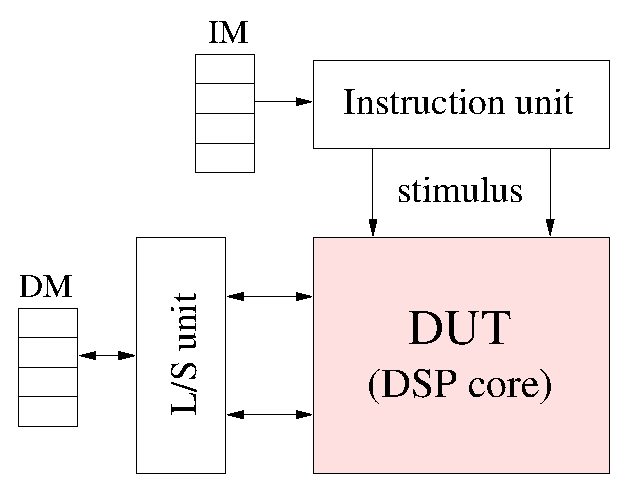
\includegraphics[width=0.6\textwidth]{./figs/sim.eps}
    \caption{Simulation environment}
    \label{fig:sim}
\end{figure}
\\\indent 
It is important to note that we focused on single-core architectures instead of the multi-core ones in the experiment.
Currently, benchmark results of multi-core systems are highly correlated with the amount of optimization applied to the interconnection and the memory subsystem~\cite{trends}.
Moreover, the programming language also plays a crucial role in multi-core system performance, 
but popular ones such as CUDA, OpenCL and OpenMP are still contending for adoption as the industry standard.
Consequently, the development of a fair benchmark for multi-core DSP platforms is still an open field of study~\cite{landscape}.
Owing to aforementioned issues, we believe benchmarking the single-core DSPs can present more objective evaluation, 
\section{Pre-synthesis Analysis}
{
    \subsection{Operations per Cycle}
    Operations per cycle (OPC) evaluates the utilization rate of the ALU.
    This metric is obtained by statically scheduling operations of a DSP kernel for various architectures.
    Under the performance requirement of target applications, OPC helps to determine the timing constraint for hardware synthesis, 
    where higher OPC brings looser timing constraint, which results in lower cost from the post-synthesis hardware.
    Table~\ref{tab:opc} profiles the OPC of the DSP cores with the assumption that every operation consumes exactly one clock cycle.
    The OPC of the scalar processor is fixed to 1.0 because of the limitation of the single-issue datapath.
    On the contrary, benefiting from the wide issue-width and large port number of RF, VLIW gains the best OPC in all benchmarks.
    \\\indent
    The OPC of DeAr is limited by the access pattern of the sequential-access banked RF, which either be LIFO or FIFO, 
    and thus it was not possible for DeAr to out-perform the VLIW in regard to OPC.
    Nevertheless, by leveraging the proposed HDFG-based scheduling,  
    DeAr still gains approximate OPC of the VLIW, with only 1.11\% and 4.26\% loss in BLAS and GDSPK respectively.
    On the other hand, the OPC of composite FU architecture is highly correlated with the cascade order and the benchmark characteristic. 
    On average, the MSA order gains better OPC than the AMS order does, 
    but the former still underperforms VLIW by 12.3\% and 17.7\% in BLAS and GDSPK respectively.
    \begin{table}[!ht]
        \centering
        \caption{Operations per cycle profiling}
        \label{tab:opc}
        \resizebox{\columnwidth}{!}
        {
            \begin{tabular}{|c|c|c|c|c|c|c|c|c|c|}
                \hline
                \multicolumn{10}{|c|}{\textbf{Basic linear algebra subprograms (BLAS)}} \\ \hline
                Benchmark  &  AXPY  &  MV  &  MM  &  MINV  &  CAXPY  &  CMV  &  CMM  &  CMINV  &  Average \\ \hline 
                VLIW  &   1.94  &   1.85  &   1.72  &   1.44  &   1.97  &   1.89  &   1.80  &   1.76  &   1.79     \\ \hline 
                %2-way VLIW  &   1.94  &   1.85  &   1.72  &   1.44  &   1.97  &   1.89  &   1.80  &   1.76  &   1.79     \\ \hline 
                DeAr  &   1.94  &   1.85  &   1.72  &   1.40  &   1.97  &   1.89  &   1.80  &   1.62  &   1.77     \\ \hline
                Composite-MSA  &   2.00  &   1.88  &   1.75  &   1.37  &   1.33  &   1.35  &   1.38  &   1.53  &   1.57     \\ \hline 
                Composite-AMS  &   1.00  &   1.00  &   1.00  &   1.02  &   1.00  &   1.00  &   1.00  &   1.04  &   1.01     \\ \hline 
                Scalar  & 1.0  & 1.0  & 1.0  & 1.0  & 1.0  & 1.0  & 1.0  & 1.0  & 1.0 \\ \hline 
                \multicolumn{10}{|c|}{\textbf{General DSP application kernels (GDSPK)}}                     \\ \hline
                Benchmark  &  FIR  &  CFIR  &  LPFIR  &  Biquad  &  IT  &  DCT  &  IMDCT  &  FFT  &  Average \\ \hline 
                VLIW  &   1.82  &   1.91  &   1.67  &   1.55  &   1.33  &   1.61  &   1.86  &   1.38  &   1.64     \\ \hline 
                %2-way VLIW  &   1.82  &   1.91  &   1.67  &   1.55  &   1.33  &   1.56  &   1.64  &   1.38  &   1.61     \\ \hline 
                %         ^fix 1.67 to 1.82              ^fix 1.42 to 1.54                                 ^ fix 1.61 to 1.62
                DeAr  &   1.82  &   1.91  &   1.67  &   1.55  &   1.33  &   1.47  &   1.46  &   1.32  &   1.57     \\ \hline 
                Composite-MSA  &   1.94  &   1.34  &   1.44  &   1.42  &   1.31  &   1.14  &   1.28  &   1.06  &   1.35     \\ \hline 
                Composite-AMS  &   1.00  &   1.00  &   1.53  &   1.21  &   1.14  &   1.61  &   1.52  &   1.27  &   1.29     \\ \hline 
                Scalar  & 1.0  & 1.0  & 1.0  & 1.0  & 1.0  & 1.0  & 1.0  & 1.0  & 1.0 \\ \hline 
            \end{tabular}
        }
    \end{table}
    \subsection{Register file access rate}
    RF access rate provides a quantitative measurement of the RF activity, 
    which makes up the majority of dynamic power dissipation in DSP cores.
    It is calculated dividing the actual number of RF file accesses by the worst case number of accesses.
    Table~\ref{tab:rpd} profiles the RF access rate of each architecture in regard to various benchmarks.
    Under the assumption of single cycle datapaths, conventional architectures, scalar and VLIW, 
    lack bypassing capability and write back the arithmetic result every cycle, 
    We refer to the RF access number of such a scenario as the worst case, 
    and thus their RF access rate is fixed to 1.0.
    On the contrary, DeAr leverages TTDB and HDFG-based scheduling to exploit data bypassing opportunities. 
    As a result, its RF access rate was reduced to 0.69 and 0.73 in BLAS and GDSPK respectively, 
    and outperforms the best configured composite-ALU, MSA, which has the RF access rate of 0.77 and 0.82 respectively in BLAS and GDSPK respectively.
    \begin{table}[!ht]
        \centering
        \caption{Register file access rate profiling}
        \label{tab:rpd}
        \resizebox{\columnwidth}{!}
        {
            \begin{tabular}{|c|c|c|c|c|c|c|c|c|c|}
                \hline
                \multicolumn{10}{|c|}{\textbf{Basic linear algebra subprograms (BLAS)}} \\ \hline
                Benchmark  &  AXPY  &  MV  &  MM  &  MINV  &  CAXPY  &  CMV  &  CMM  &  CMINV  &  Average \\ \hline 
                DeAr  &   0.67  &   0.69  &   0.71  &   0.67  &   0.67  &   0.68  &   0.70  &   0.71  &   0.69     \\ \hline
                Composite-MSA  &   0.67  &   0.69  &  0.71  &   0.82  &   0.83  &   0.83  &   0.82  &   0.77  &  0.77     \\ \hline 
                Composite-AMS  &   1.0  &   1.00  &   1.00  &   0.98  &   1.00  &   1.00  &   1.00  &   0.97  &   0.99     \\ \hline 
                VLIW  &   1.00  &   1.00  &   1.00  &   1.00  &   1.00  &   1.00  &   1.00  &   1.00  &   1.00     \\ \hline 
                %2-way VLIW  &   1.00  &   1.00  &   1.00  &   1.00  &   1.00  &   1.00  &   1.00  &   1.00  &   1.00     \\ \hline 
                Saclar  &   1.00  &   1.00  &   1.00  &   1.00  &   1.00  &   1.00  &   1.00  &   1.00  &   1.00     \\ \hline 
                \multicolumn{10}{|c|}{\textbf{General DSP kernels (GDSPK)}}                     \\ \hline
                Benchmark  &  FIR  &  CFIR  &  LPFIR  &  Biquad  &  IT  &  DCT  &  IMDCT  &  FFT  &  Average \\ \hline 
                DeAr  &   0.68  &   0.67  &  0.60  &   0.57  &   0.85  &   0.74  &   0.86  &   0.82  &   0.73     \\ \hline 
                Composite-MSA  &   0.68  &   0.83  &   0.80  &   0.80  &   0.83  &   0.87  &   0.80  &   0.92  &   0.82     \\ \hline 
                Composite-AMS  &   1.00  &   1.00  &   0.77  &   0.88  &   1.00  &   0.76  &   0.84  &   0.86  &   0.87     \\ \hline 
                VLIW  &   1.00  &   1.00  &   1.00  &   1.00  &   1.00  &   1.00  &   1.00  &   1.00  &   1.00     \\ \hline 
                %2-way VLIW  &   1.00  &   1.00  &   1.00  &   1.00  &   1.00  &   1.00  &   1.00  &   1.00  &   1.00     \\ \hline 
                Saclar  &   1.00  &   1.00  &   1.00  &   1.00  &   1.00  &   1.00  &   1.00  &   1.00  &   1.00     \\ \hline 
            \end{tabular}
        }
    \end{table}
}
\section{Synthesis Result and Analysis}
{
    In this section, we present hardware synthesis results with target throughput varying from 50 to 1000 MOPS, 
    We implemented aforementioned designs with UMC 65nm cell library, 
    and measured their area and power dissipation with Synopsys Design Compiler and Synopsys Prime Time under the throughput constraint based on Table~\ref{tab:opc}.
    Synthesis failures owing to timing violation reported by the tool would remain corresponding fields empty in figures.
    \subsection{Area}
    Figure~\ref{chart:area} shows the synthesis area of DSP cores regarding to the BLAS (a) and GDSPK (b) benchmark suites.
    The proposed DeAr save 24.5\%--21.1\% and 24.9\%--21.6\% of area in BLAS and GDSPK respectively compared with VLIW.
    The area of the VLIW architecture is dominated by RF, 
    which demands complicated interconnection among ports and registers to facilitate centralized organization.
    By contrast, DeAr, which trades off the connectivity by adopting the banked RF, can thus achieve significant area reduction.
    Since the RF access latency is not critical to both VLIW and DeAr, 
    the correlation between throughput and the save area percentage achieved by DeAr is inconspicuous.
    \\\indent Besides, DeAr reduces 21.2\%--5.6\% (BLAS) and 33.5\%--4.8\% (GDSPK) of area against composite-ALU using MSA.
    When compared with AMS, the saved percentage became 17.2\%--5.3\% (BLAS) and 10.5\%--4.7\% (GDSPK).
    Composite-ALU architectures reduces area by using fewer ports in the RF.
    Nevertheless, the area burden caused by the centralized RF still exists.
    Another drawback of composite-ALU architectures is the long critical path in ALU, 
    which leads to sharp area growth as throughput increasing.
    \\\indent Benefiting from the simplicity of its datapath, 
    scalar costs lowest area when while throughput is low.
    However, the low OPC of scalar becomes the terrible burden on gaining high throughput.
    As a result, while throughput is above 600 MOPS (BLAS) or 650 MOPS (GDSPK), 
    the area of scalar exceeds the one of DeAr, 
    and DeAr achieves the lowest area among five designs.
    \vspace{\textfig}
    \begin{figure}[!ht]
        \begin{center}
            \subfigure[BLAS benchmark suite]
            {
                \label{chart:area:blas}
                \includegraphics[width=0.48\textwidth]{charts/area_blas.eps}
            }
            \subfigure[General benchmark suite]
            {
                \label{chart:area:general}
                \includegraphics[width=0.48\textwidth]{charts/area_general.eps}
            }
        \end{center}
        \caption{Synthesis area of the DSP cores}
        \label{chart:area}
    \end{figure}
    \subsection{Power dissipation}
    The power dissipation in CMOS circuits consists of the dynamic power and static power.
    In our experiment, the former was the dominating factor, which accounted for 98\%-70\% of the total dissipation, 
    owing to the technology feature.
    As a result, we focus on the analysis of the dynamic power, 
    which is proportional to the product of clock rate $f$, logic switching rate $\alpha$ and the load $C_L$ of each cell.
    \\\indent
    Figure~\ref{chart:area} shows the power dissipation of DSP cores regarding to the BLAS~(a) and GDSPK~(b) benchmark suites.
    Generally, they grow at various slopes with throughput, which has a factor of $f$, 
    and the near-linear growth indicates the domination of the dynamic power.
    DeAr saves 22.7\%--15.1\% (BLAS) and 18.5\%--10.4\% (GDSPK) of power compared with VLIW.
    The power reduction achieved by DeAr is attributed to its low register access rate, which reduces $\alpha$
    and banked RF organization, which reduces $C_L$.
    \\\indent
    The power dissipation of composite-ALU is significantly affected by ALU order.
    Below 600 MOPS, DeAr achieves 46.9\%--41.2\% (BLAS) and 19.7\%--15.8\% (GDSPK) power reduction against AMS, 
    but only achieves 7.1\%--2.6\% (BLAS) and 11.4\%--1.5\% (GDSPK) against MSA.  
    Compared with AMS, MSA benefits from high OPC, which reduces $f$, and low RF access rate, which reduces $\alpha$, 
    so it could stay competitive against DeAr in this metric.
    However, the sharp area growth of composite-ALU also drives the severe growth of $C_L$ in the long run.
    As a result, power dissipation of MSA gradually diverges from the one of DeAr as throughput increasing, 
    and DeAr achieves 22.5\%--8.7\% (BLAS) and 37.8\%--12.1\% (GDSPK) reduction against MSA while throughput is above or equal 600 MOPS.
    \\\indent
    Although the scalar processor costs very low area, which implies very low $C_L$, 
    the worst OPC and RF access rate among designs brings unfavorable $f$ and $\alpha$, 
    which results in severe power dissipation. 
    Compared with the scalar, DeAr saves 52.1\%--45.8\% (BLAS) and 47.1\%--38.5\% (GDSPK) of power while throughput is below 700 MOPS, 
    and the synthesis for scalar failed while throughput is above 700 MOPS.
    In regard to power dissipation, DeAr achieves the best result among designs regardless of throughput.
    \vspace{\textfig}
    \begin{figure}[!ht]
        \begin{center}
            \subfigure[BLAS benchmark suite]
            {
                \label{chart:power:blas}
                \includegraphics[width=0.48\textwidth]{charts/power_blas.eps}
            }
            \subfigure[General benchmark suite]
            {
                \label{chart:power:general}
                \includegraphics[width=0.48\textwidth]{charts/power_general.eps}
            }
        \end{center}
        \caption{Power dissipation of the DSP cores}
        \label{chart:area}
    \end{figure}
    \subsection{Static Power Dissipation}
    The evaluation of static power dissipation can present rough patterns of total power dissipation in more advanced CMOS technologies, 
    where the static portion of power usually exceeds the dynamic one.
    Fig.~\ref{chart:leakage} shows the static power dissipation of DSP cores in regard to the BLAS~(a) and GDSPK~(b) benchmark suites.
    The fact that growth pattern of Fig.~\ref{chart:leakage} is similar to the one of Fig~\ref{chart:area} regardless of the design indicates a high correlation between static power and area.
    As a result, compared with VLIW, DeAr saves 30.1\%--22.7\% (BLAS) and 29.6\%--21.9\% (GDSPK) of static power, 
    which are approximate to the save percentage of area, 24.5\%--21. 1\% and 24.9\%--21.6\%.
    \\\indent 
    On the other hand, DeAr saves up to 40.3\% (BLAS) and 58.1\% (GDSPK) of static power against MSA.
    When compared with AMS, DeAr saves up to 31.2\% (BLAS) and 10.4\% (GDSPK) of static power.
    Suffering from the sharp growth of area, 
    Composite-ALU causes severer and severer power dissipation as throughput increasing.
    Accordingly, the save percentage against composite-ALU grows with throughput regardless of the benchmark suite and ALU order.
    Note that in GDSPK with throughput below 350 MOPS, 
    DeAr causes slight increase of static power (below 3\% and 4\%) compared with MSA and AMS respectively.
    Such slight increase is result from the control logic of TTDB, 
    which is the main burden of DeAr.
    \\\indent 
    Similar to the scenario in the area evaluation, 
    scalar consumes less static power than DeAr does while throughput is low.
    Nevertheless, while throughput is above 350 MOPS, DeAr saves 23.7\%--2.2\% (BLAS) and 23.4\%--2.1\% (GDSPK) of static power instead against the scalar, 
    which suffers from the sharp growth of area as well.
    As a result, DeAr achieves the lowest static power dissipation among five designs in both benchmark suites while throughput is above 350 MOPS.
    \vspace{\textfig}
    \begin{figure}[!ht]
        \begin{center}
            \subfigure[BLAS benchmark suite]
            {
                \label{chart:leakage:blas}
                \includegraphics[width=0.48\textwidth]{charts/leakage_blas.eps}
            }
            \subfigure[General benchmark suite]
            {
                \label{chart:leakage:general}
                \includegraphics[width=0.48\textwidth]{charts/leakage_general.eps}
            }
        \end{center}
        \caption{Leakage power dissipation of DSP cores}
        \label{chart:leakage}
    \end{figure}
}


